\subsection{Human--Judge Agreement}
\label{sec:human-summary}

\begin{figure*}[t]
\centering
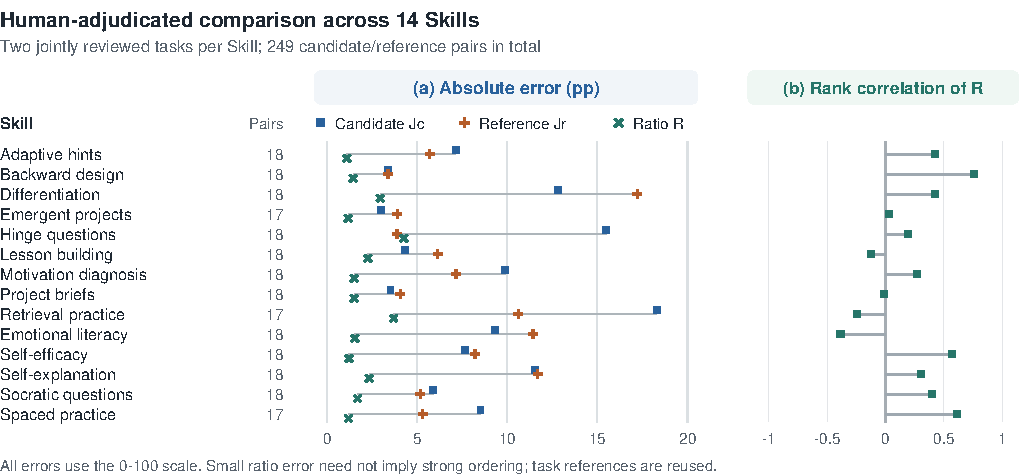
\includegraphics[width=\textwidth]{figures/human_review_v4.pdf}
\caption{Human--Judge comparison across 14 Skills: two reviewed tasks per
Skill and 249 substantive pairs. Left: candidate $J_c$, reference $J_r$,
and relative-score $R$ MAE (percentage points). Right: $R$ Spearman
correlation. References are reused within tasks; small ratio errors can
coexist with weak ordering agreement.}
\label{fig:human-breakdown}
\end{figure*}

\paragraph{Design.}
Two expert reviewers jointly adjudicated 28 tasks, two per Skill, covering
five models in both conditions. Excluding 28 reference-self and three
execution-failure controls leaves 249 candidate--reference pairs. Reviewers
use the same rubric and 0--10 scale, scoring each reference once.
Following \citet{eduillustrate}, we examine agreement by educational
dimension; here the breakdown follows 14 Skill families
(Appendix~\ref{app:human}).

\begin{table}[t]
\centering\small
\setlength{\tabcolsep}{5pt}
\begin{tabular}{lrrr}
\toprule
Score & MAE & Bias & $\rho$\\
\midrule
\inputtable{tables/full_ref_metrics.tex}
\bottomrule
\end{tabular}
\caption{249-pair agreement. MAE and human-minus-Judge bias are in
percentage points; $\rho$ is Spearman correlation.}
\label{tab:ref-human-metrics}
\end{table}

\paragraph{Score proximity and ranking differ.}
Table~\ref{tab:ref-human-metrics} shows a 1.99-point $R$ MAE, compared
with 8.61 and 7.43 for candidate and reference quality. Candidate $J$
averages 92.23 under the Judge and 86.10 after adjudication. Ratio
compression and cancellation of shared shifts can reduce this discrepancy
without validating absolute correctness or improving pointwise judging.
The $R$ correlation is 0.165; exact candidate/tie/reference agreement is
133/249 (53.41\%).

\paragraph{Disagreement is skill-specific.}
Figure~\ref{fig:human-breakdown} localizes the largest $R$ errors to
hinge questions (4.26 points) and retrieval practice (3.70), versus adaptive
hints (1.10) and emergent projects (1.17). Faulty answer keys undermine
worked solutions and student diagnoses despite plausible teaching structure.
Backward design shows stronger relative ordering ($\rho=0.756$).
These differences identify teaching operations that need closer inspection.
Each family contributes only two reviewed tasks, and the experts produce
one consensus label set rather than independent ratings. The analysis
therefore diagnoses evaluator behavior without establishing universal
reliability or resolving small leaderboard differences.
